\documentclass[aspectratio=169]{beamer}

% Theme
\usetheme{default}
\usecolortheme{beaver}

% Packages
\usepackage{amsmath,amssymb,amsthm}
\usepackage{mathtools}
\usepackage{bm}
\usepackage{tikz}
\usetikzlibrary{arrows.meta,positioning,calc}

% Custom commands
\newcommand{\R}{\mathbb{R}}
\newcommand{\Ld}{\mathcal{L}^d}
\newcommand{\Pp}{\mathcal{P}_p}

% Title
\title{Introduction to Optimal Transport}
\subtitle{From Monge to Kantorovich}
\author{}
\date{}

\begin{document}

%==============================================================================
\begin{frame}
\titlepage
\end{frame}

%==============================================================================
\begin{frame}{Outline}
\tableofcontents
\end{frame}

%==============================================================================
\section{The Monge Problem}
%==============================================================================

\begin{frame}{The Monge Problem (1781)}
Given two densities $f, g \geq 0$ on $\R^d$ with $\int f(x)\,dx = \int g(y)\,dy = 1$,\\
find a map $T: \R^d \to \R^d$ such that:
\[
\int_A g(y)\,dy = \int_{T^{-1}(A)} f(x)\,dx \quad \text{for any Borel set } A \subset \R^d
\]
minimizing the \textbf{total cost}:
\[
M(T) := \int_{\R^d} \underbrace{|T(x) - x|}_{\text{distance}} \cdot \underbrace{f(x)}_{\text{density}} \, dx
\]

\vspace{0.3cm}
\begin{center}
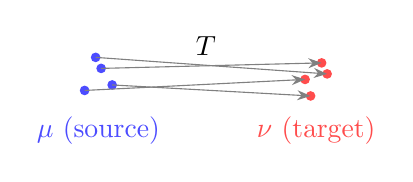
\begin{tikzpicture}[scale=0.7]
    \foreach \x/\y in {0/0, 0.3/0.4, 0.5/0.1, 0.2/0.6} {
        \fill[blue!70] (\x,\y) circle (2.5pt);
    }
    \node[below,blue!70] at (0.25,-0.3) {$\mu$ (source)};

    \foreach \x/\y in {4/0.2, 4.3/0.5, 4.1/-0.1, 4.4/0.3} {
        \fill[red!70] (\x,\y) circle (2.5pt);
    }
    \node[below,red!70] at (4.2,-0.3) {$\nu$ (target)};

    \draw[-{Stealth},gray] (0.5,0.1) -- (4.1,-0.1);
    \draw[-{Stealth},gray] (0.3,0.4) -- (4.3,0.5);
    \draw[-{Stealth},gray] (0,0) -- (4,0.2);
    \draw[-{Stealth},gray] (0.2,0.6) -- (4.4,0.3);

    \node at (2.2,0.8) {$T$};
\end{tikzpicture}
\end{center}
\end{frame}

%==============================================================================
\begin{frame}{Push-forward Measure}
For a measure $\mu$ on $X$ and a map $T: X \to Y$, the \textbf{push-forward} $T_\#\mu$ is:
\[
(T_\#\mu)(A) = \mu(T^{-1}(A)) \quad \text{for every measurable } A \subset Y
\]
Equivalently:
\[
\int_Y \phi(y) \, d(T_\#\mu)(y) = \int_X \underbrace{\phi(T(x))}_{\text{composition}} \, d\mu(x)
\]
for every measurable $\phi$.

\vspace{0.3cm}
\begin{center}
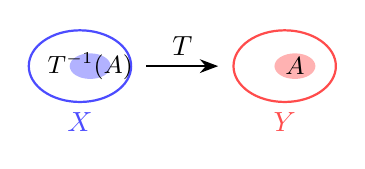
\begin{tikzpicture}[scale=0.65]
    \draw[blue!70,thick] (0,0) ellipse (1 and 0.7);
    \node[blue!70] at (0,-1.1) {$X$};
    \fill[blue!30] (0.2,0) ellipse (0.4 and 0.25);
    \node[font=\small] at (0.2,0) {$T^{-1}(A)$};

    \draw[-{Stealth},thick] (1.3,0) -- node[above] {$T$} (2.7,0);

    \draw[red!70,thick] (4,0) ellipse (1 and 0.7);
    \node[red!70] at (4,-1.1) {$Y$};
    \fill[red!30] (4.2,0) ellipse (0.4 and 0.25);
    \node[font=\small] at (4.2,0) {$A$};
\end{tikzpicture}
\end{center}
\end{frame}

%==============================================================================
\begin{frame}{General Monge Problem}
For a general cost function $c: X \times Y \to \R$:
\[
\text{(MP)} \quad \min \left\{ M(T) := \int_X \underbrace{c(x, T(x))}_{\text{cost to move } x \to T(x)} \, d\mu(x) \;:\; T_\#\mu = \nu \right\}
\]

\vspace{0.3cm}
If $\mu, \nu$ have densities $f, g$ and $T$ is smooth, injective:
\[
\underbrace{g(T(x))}_{\text{target density}} \cdot \underbrace{\det(DT(x))}_{\text{volume change}} = \underbrace{f(x)}_{\text{source density}}
\]

\vspace{0.3cm}
\textbf{Common costs:}
\begin{itemize}
    \item $c(x,y) = |x-y|$ \quad (Monge's original)
    \item $c(x,y) = |x-y|^2$ \quad (quadratic/kinetic energy)
\end{itemize}
\end{frame}

%==============================================================================
\begin{frame}{Difficulties with the Monge Problem}
\textbf{Key issue:} A map $T$ cannot split mass!

\vspace{0.3cm}
\begin{center}
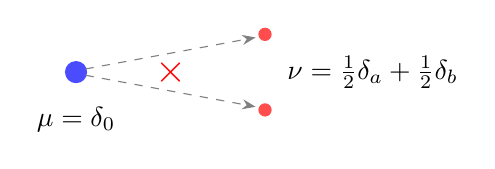
\begin{tikzpicture}[scale=0.8]
    \fill[blue!70] (0,0) circle (5pt);
    \node[below] at (0,-0.4) {$\mu = \delta_0$};

    \fill[red!70] (3,0.6) circle (3pt);
    \fill[red!70] (3,-0.6) circle (3pt);
    \node[right] at (3.2,0) {$\nu = \tfrac{1}{2}\delta_a + \tfrac{1}{2}\delta_b$};

    \draw[-{Stealth},gray,dashed] (0.15,0.05) -- (2.85,0.55);
    \draw[-{Stealth},gray,dashed] (0.15,-0.05) -- (2.85,-0.55);

    \node[red] at (1.5,0) {\Large $\times$};
\end{tikzpicture}
\end{center}

\vspace{0.2cm}
\textbf{Problems:}
\begin{itemize}
    \item Constraint $T_\#\mu = \nu$ is \textbf{nonlinear}
    \item Optimal map may \textbf{not exist}
    \item Weak convergence $T_n \rightharpoonup T$ does not imply $(T_n)_\#\mu \to T_\#\mu$
\end{itemize}

\vspace{0.2cm}
$\Rightarrow$ Problem remained unsolved for $\sim$160 years!
\end{frame}

%==============================================================================
\section{Kantorovich Relaxation}
%==============================================================================

\begin{frame}{Kantorovich's Relaxation (1942)}
\textbf{Key idea:} Replace transport \emph{maps} with transport \emph{plans}.

\vspace{0.3cm}
A \textbf{transport plan} $\gamma$ on $X \times Y$ satisfies:
\[
\underbrace{(\pi_x)_\#\gamma = \mu}_{\text{first marginal}} \quad \text{and} \quad \underbrace{(\pi_y)_\#\gamma = \nu}_{\text{second marginal}}
\]
Denote the set of all such plans by $\Pi(\mu, \nu)$.

\vspace{0.3cm}
\textbf{Kantorovich Problem:}
\[
\text{(KP)} \quad \min_{\gamma \in \Pi(\mu,\nu)} \int_{X \times Y} c(x,y) \, d\gamma(x,y)
\]

\vspace{0.3cm}
\textbf{Advantages:}
\begin{itemize}
    \item Linear objective + linear constraints $\Rightarrow$ \textbf{Linear Programming}
    \item Existence guaranteed (weak-* compactness)
    \item Mass splitting allowed!
\end{itemize}
\end{frame}

%==============================================================================
\begin{frame}{Transport Plan Visualization}
\begin{columns}
\begin{column}{0.5\textwidth}
\textbf{Monge map:}\\
$x \mapsto T(x)$ (one destination)

\vspace{0.5cm}
\textbf{Kantorovich plan:}\\
$\gamma(x,y)$ = mass from $x$ to $y$\\
(can split!)

\vspace{0.5cm}
If $T$ is a Monge map:
\[
\gamma = (\text{Id} \times T)_\#\mu
\]
is a valid plan.
\end{column}
\begin{column}{0.5\textwidth}
\begin{center}
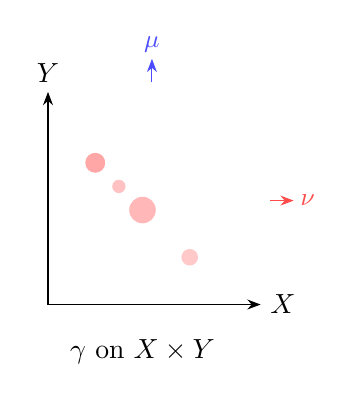
\begin{tikzpicture}[scale=0.6]
    \draw[-{Stealth}] (0,0) -- (4.5,0) node[right] {$X$};
    \draw[-{Stealth}] (0,0) -- (0,4.5) node[above] {$Y$};

    \fill[red!50,opacity=0.7] (1,3) circle (6pt);
    \fill[red!40,opacity=0.7] (2,2) circle (8pt);
    \fill[red!30,opacity=0.7] (3,1) circle (5pt);
    \fill[red!35,opacity=0.7] (1.5,2.5) circle (4pt);

    \node at (2,-1) {$\gamma$ on $X \times Y$};

    \draw[-{Stealth},blue!70] (2.2,4.7) -- (2.2,5.2);
    \node[blue!70,font=\small] at (2.2,5.5) {$\mu$};

    \draw[-{Stealth},red!70] (4.7,2.2) -- (5.2,2.2);
    \node[red!70,font=\small] at (5.5,2.2) {$\nu$};
\end{tikzpicture}
\end{center}
\end{column}
\end{columns}
\end{frame}

%==============================================================================
\section{Brenier's Theorem}
%==============================================================================

\begin{frame}{Brenier's Theorem (1991)}
For the \textbf{quadratic cost} $c(x,y) = |x-y|^2$:

\vspace{0.3cm}
\textbf{Theorem (Brenier):} If $\mu \ll \Ld$ (absolutely continuous), then:
\begin{enumerate}
    \item There exists a \textbf{unique} optimal transport map $T$
    \item $T = \nabla u$ for some \textbf{convex function} $u: \R^d \to \R$
\end{enumerate}

\vspace{0.3cm}
\begin{center}
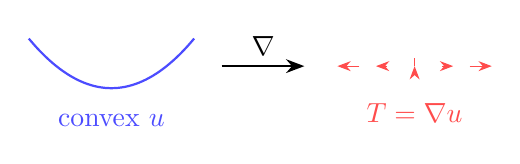
\begin{tikzpicture}[scale=0.7]
    \draw[thick,blue!70] plot[smooth,domain=-1.5:1.5] (\x,{0.4*\x*\x});
    \node[below,blue!70] at (0,-0.3) {convex $u$};

    \draw[-{Stealth},thick] (2,0.4) -- node[above] {$\nabla$} (3.5,0.4);

    \begin{scope}[shift={(5.5,0.4)}]
        \foreach \x in {-1,-0.5,0,0.5,1} {
            \draw[-{Stealth},red!70] (\x,0) -- ({\x+0.4*\x},0);
        }
        \node[below,red!70] at (0,-0.5) {$T = \nabla u$};
    \end{scope}
\end{tikzpicture}
\end{center}

\vspace{0.2cm}
The optimal transport is the \textbf{gradient of a convex function}.
\end{frame}

%==============================================================================
\begin{frame}{Monge-Amp\`ere Equation}
Combining the Jacobian equation with $T = \nabla u$:
\[
g(\nabla u(x)) \cdot \det(D^2 u(x)) = f(x)
\]
Rearranging:
\[
\det\bigl(\underbrace{D^2 u(x)}_{\text{Hessian}}\bigr) = \frac{f(x)}{g(\nabla u(x))}
\]

\vspace{0.3cm}
This is the \textbf{Monge-Amp\`ere equation}:
\begin{itemize}
    \item Fully nonlinear elliptic PDE
    \item Well-posed in the class of \textbf{convex functions}
    \item Rich regularity theory (Caffarelli, 1990s)
\end{itemize}

\vspace{0.3cm}
\textbf{Polar Factorization:} Any $v: \R^d \to \R^d$ can be written as $v = \nabla u \circ s$ where $u$ is convex and $s$ is measure-preserving.
\end{frame}

%==============================================================================
\section{Wasserstein Distance}
%==============================================================================

\begin{frame}{Wasserstein Distance}
\textbf{Definition:} For probability measures $\mu, \nu$ and $p \geq 1$:
\[
W_p(\mu, \nu) := \left( \inf_{\gamma \in \Pi(\mu,\nu)} \int_{X \times Y} \underbrace{|x-y|^p}_{\text{cost}} \, d\gamma(x,y) \right)^{1/p}
\]

\vspace{0.3cm}
\textbf{Properties:}
\begin{itemize}
    \item $W_p$ is a \textbf{metric} on $\Pp(\R^d) = \{\mu : \int |x|^p \, d\mu < \infty\}$
    \item Metrizes weak convergence + convergence of $p$-th moments
    \item For $p=2$ (Brenier): $W_2^2(\mu,\nu) = \int |x - \nabla u(x)|^2 \, d\mu$
\end{itemize}

\vspace{0.3cm}
\begin{center}
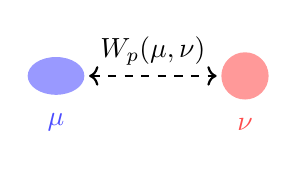
\begin{tikzpicture}[scale=0.6]
    \fill[blue!40] (0,0) ellipse (0.6 and 0.4);
    \node[below,blue!70] at (0,-0.6) {$\mu$};

    \fill[red!40] (4,0) ellipse (0.5 and 0.5);
    \node[below,red!70] at (4,-0.7) {$\nu$};

    \draw[<->,dashed,thick] (0.7,0) -- node[above] {$W_p(\mu,\nu)$} (3.4,0);
\end{tikzpicture}
\end{center}
\end{frame}

%==============================================================================
\begin{frame}{Geodesics in Wasserstein Space}
The \textbf{geodesic} from $\mu_0$ to $\mu_1$ in $(\Pp_2, W_2)$:
\[
\mu_t = \bigl(\underbrace{(1-t)\text{Id} + t\nabla u}_{\text{linear interpolation of positions}}\bigr)_\# \mu_0, \quad t \in [0,1]
\]
where $\nabla u$ is the optimal map from $\mu_0$ to $\mu_1$.

\vspace{0.3cm}
\begin{center}
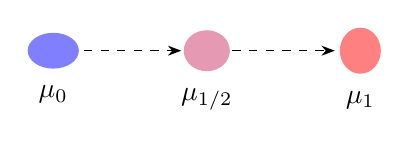
\begin{tikzpicture}[scale=0.65]
    \fill[blue!50] (0,0) ellipse (0.5 and 0.35);
    \node[below] at (0,-0.5) {$\mu_0$};

    \fill[purple!40] (3,0) ellipse (0.45 and 0.4);
    \node[below] at (3,-0.55) {$\mu_{1/2}$};

    \fill[red!50] (6,0) ellipse (0.4 and 0.45);
    \node[below] at (6,-0.6) {$\mu_1$};

    \draw[-{Stealth},dashed] (0.6,0) -- (2.5,0);
    \draw[-{Stealth},dashed] (3.5,0) -- (5.5,0);
\end{tikzpicture}
\end{center}

\vspace{0.2cm}
\textbf{Displacement interpolation:} Particles move along straight lines at constant speed.

\vspace{0.2cm}
\textbf{McCann's Displacement Convexity (1997):}
\[
\mathcal{F}(\mu_t) \leq (1-t)\mathcal{F}(\mu_0) + t\mathcal{F}(\mu_1)
\]
for many functionals $\mathcal{F}$.
\end{frame}

%==============================================================================
\section{Gradient Flows}
%==============================================================================

\begin{frame}{Gradient Flows in Wasserstein Space}
\textbf{Key insight:} Many PDEs are gradient flows in $(\Pp_2, W_2)$.

\vspace{0.3cm}
\textbf{Gradient flow} of functional $\mathcal{F}$:
\[
\partial_t \rho = -\text{grad}_{W_2} \mathcal{F}(\rho)
\]

\vspace{0.3cm}
\textbf{Example: Heat equation}
\[
\partial_t \rho = \Delta \rho
\]
is the gradient flow of the \textbf{entropy}:
\[
\mathcal{F}(\rho) = \int_{\R^d} \underbrace{\rho(x) \log \rho(x)}_{\text{entropy density}} \, dx
\]

\vspace{0.3cm}
\textbf{Other examples:}
\begin{itemize}
    \item Porous medium: $\mathcal{F}(\rho) = \frac{1}{m-1}\int \rho^m$
    \item Fokker-Planck: $\mathcal{F}(\rho) = \int \rho \log \rho + \int V \rho$
\end{itemize}
\end{frame}

%==============================================================================
\begin{frame}{JKO Scheme}
\textbf{Jordan-Kinderlehrer-Otto (1998):} Discrete-time approximation.

\vspace{0.3cm}
\[
\rho^{n+1} = \arg\min_\rho \left\{ \underbrace{\frac{1}{2\tau} W_2^2(\rho, \rho^n)}_{\text{stay close to } \rho^n} + \underbrace{\mathcal{F}(\rho)}_{\text{minimize energy}} \right\}
\]

\vspace{0.3cm}
As $\tau \to 0$:
\[
\rho^n \longrightarrow \rho(n\tau) \quad \text{solving } \partial_t \rho = -\text{grad}_{W_2}\mathcal{F}
\]

\vspace{0.5cm}
\textbf{Applications:}
\begin{itemize}
    \item Existence proofs for PDEs
    \item Numerical schemes
    \item Stability and uniqueness results
\end{itemize}
\end{frame}

%==============================================================================
\section{Geometry and Curvature}
%==============================================================================

\begin{frame}{Entropy and Ricci Curvature}
\textbf{Remarkable connection} (Lott-Villani, Sturm, 2006-2009):

\vspace{0.3cm}
On a Riemannian manifold $(M,g)$:
\[
\underbrace{E(\rho) = \int \rho \log \rho}_{\text{entropy}} \text{ is geodesically convex in } W_2
\]
\[
\Updownarrow
\]
\[
\text{Ricci curvature} \geq 0
\]

\vspace{0.3cm}
\textbf{Synthetic Ricci curvature:} For metric measure spaces $(X,d,m)$:
\[
\text{Ric} \geq K \quad \Leftrightarrow \quad \text{Entropy is } K\text{-convex along } W_2\text{-geodesics}
\]

\vspace{0.3cm}
This extends curvature bounds to \textbf{non-smooth spaces}.
\end{frame}

%==============================================================================
\section{Applications}
%==============================================================================

\begin{frame}{Applications of Optimal Transport}
\textbf{Image Processing:}
\begin{itemize}
    \item Color transfer
    \item Shape interpolation via $W_2$ geodesics
    \item Wasserstein barycenters: $\bar\mu = \arg\min_\mu \sum_i \lambda_i W_2^2(\mu, \mu_i)$
\end{itemize}

\vspace{0.3cm}
\textbf{Machine Learning:}
\begin{itemize}
    \item Wasserstein GANs
    \item Domain adaptation
    \item Distributional distances
\end{itemize}

\vspace{0.3cm}
\textbf{Economics \& Traffic:}
\begin{itemize}
    \item Spatial economics (supply/demand allocation)
    \item Traffic congestion: $\min \int g(\rho) |v| \, dx\,dt$
    \item Branched transport: subadditive costs $m^\alpha$ ($0 < \alpha < 1$)
\end{itemize}
\end{frame}

%==============================================================================
\section{Computational Methods}
%==============================================================================

\begin{frame}{Computational Methods}
\textbf{1. Linear Programming:}
\begin{itemize}
    \item Exact for discrete measures
    \item Hungarian algorithm: $O(n^3)$
\end{itemize}

\vspace{0.3cm}
\textbf{2. Entropic Regularization} (Cuturi, 2013):
\[
\min_{\gamma \in \Pi(\mu,\nu)} \int c \, d\gamma + \underbrace{\varepsilon \int \gamma \log \gamma}_{\text{entropy penalty}}
\]

\begin{itemize}
    \item \textbf{Sinkhorn algorithm:} Iterative matrix scaling
    \item Nearly linear complexity
    \item Differentiable $\Rightarrow$ deep learning applications
\end{itemize}

\vspace{0.3cm}
\textbf{3. Semi-discrete methods:}
\begin{itemize}
    \item One continuous, one discrete measure
    \item Laguerre tessellation / power diagrams
\end{itemize}
\end{frame}

%==============================================================================
\begin{frame}{Summary}
\textbf{Theory:}
\begin{itemize}
    \item Monge (1781): Transport maps, $\min \int |T(x)-x| f(x)\,dx$
    \item Kantorovich (1942): Transport plans, linear programming
    \item Brenier (1991): $T = \nabla u$ for quadratic cost
\end{itemize}

\vspace{0.3cm}
\textbf{Geometry:}
\begin{itemize}
    \item Wasserstein distance $W_p$
    \item Geodesics, displacement convexity
    \item Gradient flows for PDEs
    \item Ricci curvature bounds
\end{itemize}

\vspace{0.3cm}
\textbf{Computation:}
\begin{itemize}
    \item Sinkhorn algorithm (entropic regularization)
    \item GPU-accelerated methods for ML
\end{itemize}
\end{frame}

%==============================================================================
\begin{frame}{References}
\textbf{Books:}
\begin{itemize}
    \item C. Villani, \textit{Optimal Transport: Old and New}, Springer 2009
    \item F. Santambrogio, \textit{Optimal Transport for Applied Mathematicians}, 2015
    \item G. Peyr\'e \& M. Cuturi, \textit{Computational OT}, Found.\& Trends ML, 2019
\end{itemize}

\vspace{0.3cm}
\textbf{Key papers:}
\begin{itemize}
    \item Y. Brenier, \textit{Polar factorization...}, CPAM 1991
    \item R. Jordan, D. Kinderlehrer, F. Otto, SIAM 1998
    \item M. Cuturi, \textit{Sinkhorn Distances}, NeurIPS 2013
\end{itemize}
\end{frame}

%==============================================================================
\begin{frame}
\begin{center}
\Huge Thank You!

\vspace{1cm}
\Large Questions?
\end{center}
\end{frame}

\end{document}
